\documentclass[11pt]{article}
\usepackage{fullpage}
\usepackage{geometry}                % See geometry.pdf to learn the layout options. There are lots.
\geometry{letterpaper}                   % ... or a4paper or a5paper or ... 
%\geometry{landscape}                % Activate for for rotated page geometry
%\usepackage[parfill]{parskip}    % Activate to begin paragraphs with an empty line rather than an indent
\usepackage{graphicx}
\usepackage{amssymb}
\usepackage{amsmath}
\usepackage{epstopdf}
\DeclareGraphicsRule{.tif}{png}{.png}{`convert #1 `dirname #1`/`basename #1 .tif`.png}



\title{}
\author{}
\date{}                                           % Activate to display a given date or no date

\begin{document}
\maketitle
%\section{}
%\subsection{}

\section{Random Harvard IDs}
First imagine there are two people in the room. There is a $\frac{1}{10}$ probability that the two IDs match at the $i$th digit. For any substring of length $k$ in the ID, the probability that all $k$ digits match is $\frac{1}{10^{k}}$. Conversely, the probability that the two substrings differ somehow is $1 - \frac{1}{10^{k}}$. \\
\\
Now consider increasing numbers of people in the room. Assuming that the first two people do not duplicate each other on a given $k$-length substring, there are two different substrings present when the third person enters. Therefore the third person duplicates one of the substrings with probability $\frac{2}{10^{k}}$. So the total probability that the three substrings do not duplicate each other is
$\left ( 1 - \frac{1}{10^{k}} \right )  \left (1 -  \frac{2}{10^{k}} \right )$. Generally, when there are $n$ people in the room the probability that all $k$-length substrings differ is $\left ( 1 - \frac{1}{10^{k}} \right )  \left (1 -  \frac{2}{10^{k}} \right ) \cdots  \left (1 - \frac{n-1}{10^{k}} \right )$
\\
\\
Thus the questions below require the value of $n$ that makes this equation drop below $\frac{1}{2}$ for different values of $k$.
\\
\begin{itemize}
\item How many people would you need to have in a room before it was more likely than not that two had the same last four digits? \\
$k = 4 \Rightarrow n = 119$ \\
Each digit is independent. In particular the probability that an $m$ digit ID has the same last four digits as some other $m$ digit ID is the same regardless of $m$.
\item How many numbers could be issued before it would be more likely than not that there is a duplicate Harvard ID number? \\
$k = 8 \Rightarrow n = 11775$ \\
In this case the substring is the full ID.
\item What would the answers for the above questions be if there were 12 digit ID numbers?
$k = 4 \Rightarrow n = 119$ \\
$k = 12 \Rightarrow n = 1177411$
\end{itemize}

\section{Hash collision probabilities}
Suppose each person gets a random hash value from the range $[1 \dots n]$.
\begin{itemize}
\item Show that for some constant $c_1$, when there are at least $c_1 \sqrt{n}$ people in a room, the probability that no two have the same hash value is at most $1/e$. \\
\\
Just as with birthdays where $n = 365$, the probability that $k$ people in a room all have different hash values is $P(k) = \left (1 - \frac{1}{n} \right )\left (1 - \frac{2}{n} \right ) \cdots \left (1 - \frac{k-1}{n} \right )$.
Using the fact $e^{-x} \ge 1 - x$, it follows that $P(k) \le e^{-\frac{1}{n}} \ e^{-\frac{2}{n}} \ \cdots \ e^{-\frac{k-1}{n}} = e^{-(\frac{1}{n} + \frac{2}{n} + \cdots + \frac{k-1}{n})}$. \\
The quantity $e^{-(\frac{1}{n} + \frac{2}{n} + \cdots + \frac{k-1}{n})}$ is less than or equal to $1/e$ if $\sum_1^k \ge n$. Therefore we need to choose $c_1$ so that $k = c_1 \sqrt{n} - 1$ satisfies that inequality. \\
\\
Using the summation formula we need $\sum_1^{c_1 \sqrt{n} - 1} = \frac{(c_1 \sqrt{n} - 1)c_1 \sqrt{n}}{2} \ge n$. \\
Solving for  $c_1$ yields  $\frac{1 + \sqrt{8n + 1}}{2 \sqrt{n}} \ \ \blacksquare $
\item Show that for some constant $c_2$ (and sufficiently large $n$) when there are at most $c_2 \sqrt{n}$ people in the room, the probability that no two have the same hash value is at least $1/2$. \\
\\
Again the probability that no two people have the same hash value is $P(k) = \left (1 - \frac{1}{n} \right )\left (1 - \frac{2}{n} \right ) \cdots \left (1 - \frac{k-1}{n} \right )$. \\
\\
Using the fact that $e^{-x-x^{2}} \le 1 - x$ for $x \le \frac{1}{2}$ it follows that \\ 
$P(k) \ge e^{- \frac{1}{n} - \left ( \frac{1}{n} \right )^{2}} \ e^{- \frac{2}{n} - \left ( \frac{2}{n} \right )^{2}} \cdots e^{- \frac{k}{n} - \left ( \frac{k}{n} \right )^{2}}$ assuming that $k \le n/2$. \\
\\
Because $e^{-x} \ge e^{-y}$ when $x \le y$, the equation above implies that \\
$P(k) \ge e^{k \left (- \frac{k}{n} - \left ( \frac{k}{n} \right )^{2} \right )} \ge e^{k \left (-2 \frac{k}{n} \right )}$.
Note that $\frac{k}{n} \ge \frac{k^{2}}{n^{2}}$ when $k \le n$.
\\
\\
So we need to choose $k = c_2 \sqrt{n} - 1$ so that $e^{-2 \left ( \frac{k^{2}}{n} \right )} \ge 1/2$. \\
This means $-2 \left ( \frac{k^{2}}{n} \right ) \ge -ln\ 2$, or that $2 \left ( \frac{k^{2}}{n} \right ) \le ln\ 2$. \\
Solving yields $k \le \sqrt{ \frac{n\,ln\ 2}{2}}$; setting $k = c_2 \sqrt{n} - 1$ and solving for $c_2$ gives \\ $c_2 \le \sqrt{ \frac{ln\ 2}{2}} + \frac{1}{\sqrt{n}}$. \\


To maximize the number of people in the room, set $c_2 = \sqrt{ \frac{ln\ 2}{2}} + \frac{1}{\sqrt{n}} \ \ \blacksquare $
\end{itemize}

\section{Document Similarity}
Assume that $D$ and $E$ are two documents, and we have created 84 element original sketches for both and divided each sketch into 6 groups of 14 permutations, $G_{1D} \dots G_{6D}$ and $G_{1E} \dots G_{6E}$. Consider one pair of these groups, say $G_{1D}, G_{1E}$. 
\\
\\
If it happens that all 14 elements match then the super-sketch values will agree, because they will agree on all 14 of the re-hashed values, and thus they will agree on the minimum of that set. It is possible that the super-sketch values will agree if fewer than 14 elements match. Say 13 out of 14 values match - then the super-sketch values will match with probability 13/14. Even if only 1 out of the 14 elements matches it is possible that this value will be the minimum after re-hashing.
\\
\\
Nevertheless, it is reasonable to interpret a match in a pair of super-sketch values to mean that the 14 elements in the original sketch matched. Because the resemblance of $D$ and $E$ is $r$, we expect that $14 r$ of the elements match between the two groups. When we have $14r$ matches, the resulting super-sketch values will agree with probability $r$. Since the super-sketch creation encodes the resemblance, if two super-sketch values match then they are a proxy for matches in the original sketch. The super-sketch is like flipping a coin with probability $r$ of heads, and if we get heads we call it a match.
\\
\\
To make this more precise: the probability of $i$ matches among the 14 original sketch values in $G_{1D}$ and $G_{1E}$ is $\binom{14}{i} r^i(1-r)^{14-i}$. When there are $i$ matches the probability that the corresponding super-sketches match is $i/14$. Thus the total probability that the super-sketches match is $\sum_0^{14} \binom{14}{i} r^i(1-r)^{14-i} \left ( \frac{i}{14} \right )$. This sum is equal to $r$. (The ruby program at the end of this discussion demonstrates that empirically.)
\\
\\
Therefore the probability of 2 or more matches among the 6 pairs of super-sketches for $D$ and $E$ is $\sum_2^{6} r^i(1-r)^{6-i}$. It turns out that if the resemblance is over 0.5 then there is at least a  90\% probability that 2 or more super-sketches will match. When resemblance is 0.25 there is roughly a 50\% chance of 2 or more super-sketch matches. \\
\\
The graph on the next page shows the full results. \\
\\
Also, qualitatively the likelihood of collisions on both hashing steps is greater when using 16 or 8 bits instead of 64, so documents are more likely to be flagged as duplicates. Quantitatively it seems like the number of collisions we get depends on document length, the document content, and the precise mechanics of how k-word groups are hashed to n-bit numbers. Independent of those details though, moving from 64 bits to 16 bits reduces the number of hash values from $2^{64}$ to $2^{16}$, increasing the likelihood of collisions by a factor of $2^{48}$. For 8 bits that factor is $2^{56}$.

\newpage
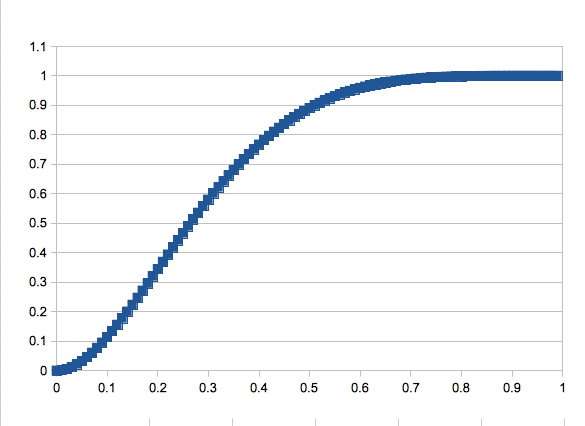
\includegraphics[width=150mm,height=120mm]{super-sketch.png}

This graph shows resemblance on the horizontal axis and probability of 2 or more out of 6 matches on the vertical. The data was generated by the last part of the program on the following page. It computes the probability for values of $r$ from 0.01 to 1.0, ascending in 0.01 step increments.

\newpage

\begin{verbatim}
class Integer
  def choose(k)   # binomial coefficient: n C k
    pTop = (self-k+1 .. self).inject(1, &:*) # n!/(n-k)!
    pBottom = (2 .. k).inject(1, &:*)  # k!
    pTop / pBottom
  end
end

# experimentally show that probability of super-sketch matches is r
r = 0.9
max = 14
p = 0
i = 0
while i <= max do
    eq1 = max.choose(i)
    eq2 = r**i
    eq3 = (1-r)**(max-i)
    eq4 = i / Float(max)
    p += eq1 * eq2 * eq3 * eq4
    puts "#{i}\t#{p}"
    i = i+1
end
puts ""

# calculate probability of 2 of more super-sketch across a range of r values
r = 0.01
max = 6
while r <= 1.0 do
    p = 0
    i = 2
    while i <= max do
        eq1 = max.choose(i)
        eq2 = r**i
        eq3 = (1-r)**(max-i)
        p += eq1 * eq2 * eq3
        i = i+1
    end
    puts "#{r}\t#{p}"
    r += 0.01
end
\end{verbatim}


\section{Fingerprint matching} 

\section{Primality}
As discussed in the Lecture 13 notes, a value of $a$ in which $a^{n-1} \ne 1$ mod $n$ is a witness that $n$ is composite. I wrote a program to compute $2^{636127-1}$ mod $636127$, and obtained 195504. Since that is different from 1, 2 is a witness that 636127 is composite. 
\\
\\
294409 is a Carmichael number; for example if $a = 2$, $a^{294408}$ mod 294409 = 1. \\
Using the Rabin method we can show that it is composite. \\
It is a fact that $n - 1 = 294408 = 2^t u = 2^3 * 73602$. \\
Using $u = 73602$, we find $a^{u}$ mod 294409 = 262144 $\ne \pm 1$, but for $2u = 147204$ we get \\
$a^{2u}$ mod 294409 = 1. \\
That is, we find a non-trivial square root of 1 modulo $n$, so $n$ is composite with 2 as a witness.
\section{RSA}
The binary representation of ``Give me an A'' denoted by $x$ is \\
100011111010011110110110010101000001101101110010101000001100001110111001000001000001 \\
\\
Your public key is $(n,e) = (46947848749720430529628739081,37267486263679235062064536973)$. \\
\\
Hence the encoded message is (in decimal)
\begin{equation*}
e(x) = x^{e}\ \mbox{mod}\ n = 41205849232150842891029277111
\end{equation*}



\end{document}  
